\subsection{Beschreibung HMI - Visualisierung}
\label{kap:ClientGraphProgrammVisu}
DUrch das Betätigen des Buttons \textit{Show graph} innerhalb der Hauptansicht des Programms, erfolgt das Darstellen der Visualisierung.\\
Das Visualisieren der Sensorwerte erfolgt durch vier Diagramme pro Sensor (s. Abbildung \ref{fig:clientgraphdiagramm}), in denen die Beschleunigungswerte in jeder Achse einzeln und einmal alle zusammen dargestellt werden. 
Die Auswahl des Sensors erfolgt durch einen Up-Down-Selector (s. Abbildung - Pos. 2) und das Erstellen eines Abbilds durch das Betätigen des Buttons \textit{Snapshot}. Dieses wird auf dem Desktop abgelegt.

\begin{figure}[H]
\centering
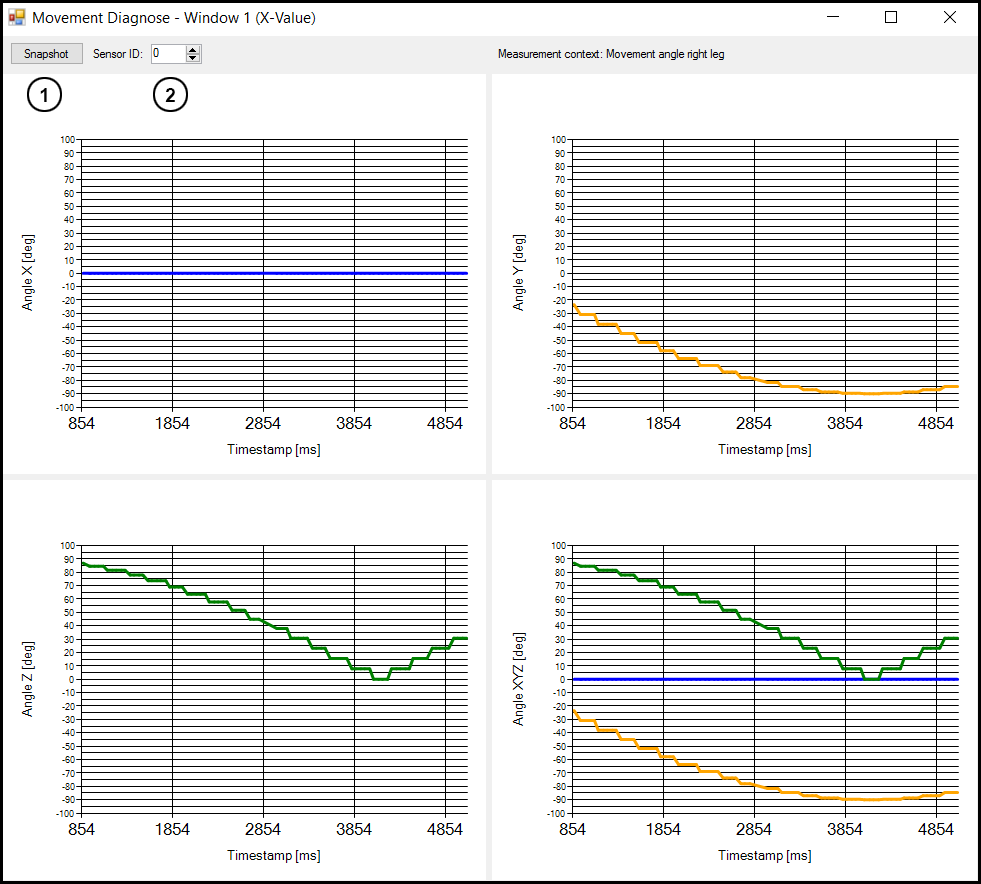
\includegraphics[width=1\linewidth]{Bilder/ClientGraphDiagramm}
\caption[Diagramm Sensorwerte]{Diagramm der Sensorwerte}
\label{fig:clientgraphdiagramm}
\end{figure}



